\documentclass[a4paper,11pt]{article}
\usepackage{graphicx}
\usepackage{amsmath}
\usepackage[colorlinks=true, linkcolor=black, citecolor=black, urlcolor=black, filecolor=black]{hyperref}
\usepackage{geometry}
\usepackage{natbib}
\usepackage{project}
\usepackage{tikz}
\usetikzlibrary{positioning, shapes.geometric, arrows}

\geometry{margin=1in}


\title{Interlinked Dynamics: Exploring the Correlations between Surface Temperature, Atmospheric CO2, Sea Level Rise, and Land Cover Changes}
\author{Hassan Ahmed (23069970)}
\date{\today}

\begin{document}

\maketitle

\section{Introduction}
Climate change is a critical issue which has to be assessed in different contexts of the environment.
This report investigates two main questions:
\begin{itemize}
    \item How do changes in atmospheric \(\text{CO}_2\) concentrations correlate with changes in sea level rise over time?
    \item Is there a correlation between rising mean surface temperatures and land cover changes?
\end{itemize}
Knowledge of climate change implications on the social sphere is imperative toward formulation of the policy and adaptations.

\section{Used Data}
\subsection{Description of Data Sources}
\begin{itemize}

\item \textbf{Dataset 1: Annual Surface Temperature Change}

This data source provides the mean surface temperature change for the period 1961–2021 for each country. It uses temperatures from 1951 and 1980 as a baseline. \cite{dataset1}

\item \textbf{Dataset 2: World Monthly Atmospheric \(\text{CO}_2\) Concentrations}

In this data source, world-wide average concentrations of \(\text{CO}_2\) are present, which have been observed on a monthly basis since 1958. \cite{dataset2}

\item \textbf{Dataset 3: Change in Mean Sea Levels}

The indicator provided in this data source is global sea level rise for different seas and oceans, observed monthly since 1993. \cite{dataset3}

\item \textbf{Dataset 4: Land Cover Altering Indicator}

This data source looks at the changes in land cover over time from 1992 to 2020 for each country. The indicator is grouped into categories on the basis of climate influence: altering, regulating, and neutral. \cite{dataset4}

\end{itemize}

\subsection{Data Structure and Quality}
\begin{itemize}
    \item \textbf{Annual Surface Temperature Change} The data is structured in a time series for each country in a horizontal manner. Temperature change is in degree-Celsius units. The main columns to use are country, iso3 (i.e., country code mapping required for generating maps), and indicator values for all the years. At most, 8\% of the data in one of the years is unobserved, which is fine as that can be imputed with zeros.

    \item \textbf{World Monthly Atmospheric \(\text{CO}_2\) Concentrations} This indicator of \(\text{CO}_2\) concentration is structured in a global time series with a monthly frequency. The main columns are date and value. The indicator value is expressed in parts per million (ppm). Nulls are 0\% in this dataset.

    \item \textbf{Change in Mean Sea Levels} In this dataset main columns are measure, date and value in millimeters. It is again a time series observed with a monthly frequency but it is categorized into major seas and oceans in measure column. There are 0\% nulls in this dataset.

    \item \textbf{Land Cover Altering Indicator} This dataset is the land cover estimation of each country into three main categories of climate influence: altering, regulating, and neutral. Annual values are in a time series for each country in horizontal manner. At most 0.3\% of the data in one of the years is unobserved, which is fine as that can be imputed with zeros.

\end{itemize}

\subsection{Licenses and Permissions}
The data sources are publicly available on \href{https://climatedata.imf.org/}{IMF} under open-data licenses. Detailed license information can be found at:
\href{https://www.imf.org/external/terms.htm}{License}

\subsection{Data Pipeline}
The data pipeline has three main modules: extractor, transform, and loader. Each of the modules has their respective functions.
First \texttt{extract\_csv} from extractor module is used to extract the data source from URL, then \texttt{delete\_columns} from transform module deletes the list of useless columns specified for every dataset, then a flag of "date\_column" is present in configs which only applies \texttt{standardize\_date\_column} to standardize the date format across necessary datasets, then renaming of the date columns is done using \texttt{rename\_year\_columns} function, it is only triggered for those datasets where flag  of "rename\_year\_columns" is equals to true, once all the transformations have been applied, dataset is then loaded to sqlite database using \texttt{load\_df\_to\_sqlite} from loader module. This can be see in figure \ref{fig:etl_pipeline}.


\begin{figure}[ht!]
    \centering
    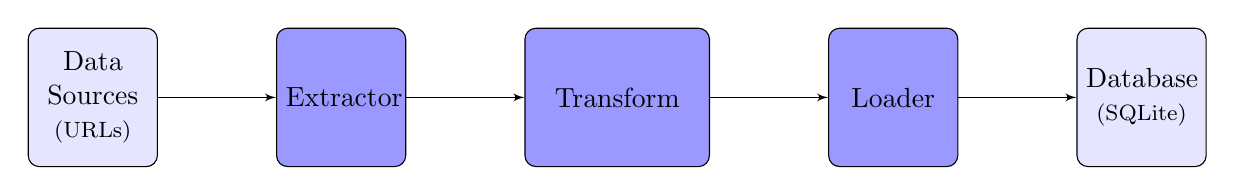
\begin{tikzpicture}[node distance=1.5cm and 1.5cm, auto]
        % Styles
        \tikzstyle{smallblock} = [rectangle, draw, fill=blue!10,
            text width=4em, text centered, rounded corners, minimum height=5em]
        \tikzstyle{block} = [rectangle, draw, fill=blue!40,
            text width=4em, text centered, rounded corners, minimum height=5em]
        \tikzstyle{largeblock} = [rectangle, draw, fill=blue!40,
            text width=6em, text centered, rounded corners, minimum height=5em]
        \tikzstyle{line} = [draw, -latex', shorten >=0pt, shorten <=0pt]

        % Nodes
        \node [smallblock] (source) {Data Sources \\ \footnotesize (URLs)};
        \node [block, right=of source] (extractor) {Extractor};
        \node [largeblock, right=of extractor] (transform) {Transform};
        \node [block, right=of transform] (loader) {Loader};
        \node [smallblock, right=of loader] (database) {Database \\ \footnotesize (SQLite)};

        % Connections
        \path [line] (source) -- (extractor);
        \path [line] (extractor) -- (transform);
        \path [line] (transform) -- (loader);
        \path [line] (loader) -- (database);
    \end{tikzpicture}
    \caption{ETL Pipeline Diagram.}
    \label{fig:etl_pipeline}
\end{figure}


\subsection{Output of Data Pipeline}
Output datasets of the pipeline for all data sources are stored in sqlite database as tables as it was faster and easier to handle as a collective database, The pipeline is coded in a way that data quality dimensions were of the upmost priority and that the output datasets of the pipeline
\begin{itemize}
    \item reflect the real word and are correct indicators
    \item contain all necessary information which is required to answer selected questions
    \item are consistent in their formats
    \item time period of datasets are appropriate and intersecting
    \item presentation of the datasets aligns with the requirements of the questions need to be answered
\end{itemize}

Annual surface temperature change and land cover altering indicator can be compared and checked for correlation and similarly the other two datasets can be compared. The only limitation is in the sea level dataset where the measure column is not friendly to be mapped on the world map for oceans and seas and no code mappings were found for them.

\section{Analysis}

Data pipeline was used to import and perform all the data engineering task before the analysis was started. The analysis was started with exploring each dataset individually and by doing so found few very exciting insights, when average temperature change was plotted on world scale and compared country wise wee found that countries in the Northern Hemisphere, especially those in the higher latitudes like Russia and Canada, exhibit the most significant increases in temperature. This occurrence also tends to support some established theories in the climate science literature in that polar regions are thought to be warming more than the rest of the globe because of changes in albedo and an enhancement of polar amplification. Those in the region of the equator receive average variations in temperature. Over the past one hundred years, Russia has experienced the largest increase in temperature; some region lies in the tropical zone records the minimum degree of change. This can be seen in figure \ref{fig:temp_change}.

\begin{figure}[ht!]
    \centering
    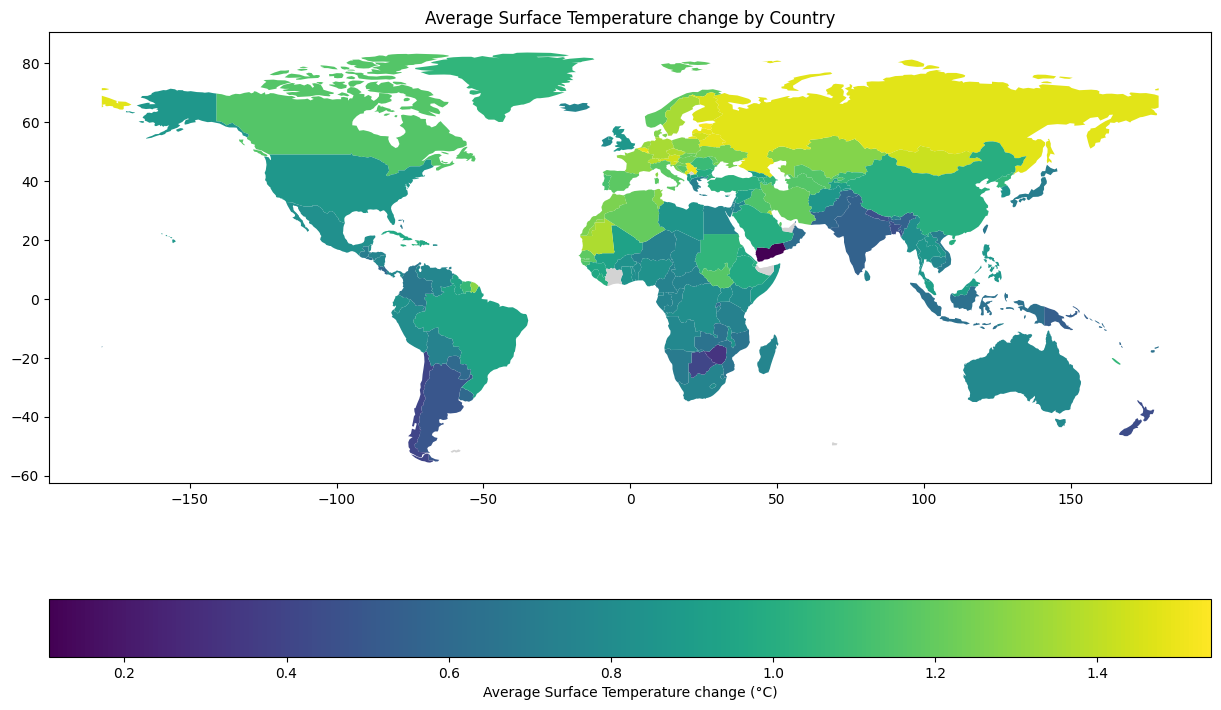
\includegraphics[width=1\textwidth]{pictures/temp_world.png}
    \caption{Average Surface Temperature Change by Country.}
    \label{fig:temp_change}
\end{figure}

By looking at the fluctuations of the sea level over the years in figure \ref{fig:sea_levels}, as it clearly indicates the trend of a rise in the average sea levels from the year 1993 to the year 2021. The trend demonstrates that the impact of both thermal expansion and melting of ice caps is causing sea levels to rise all over the globe. The latter underlines the continual growth of this phenomenon, thus stressing the consequences on the coastal zones of international scale.

\begin{figure}[h]
    \centering
    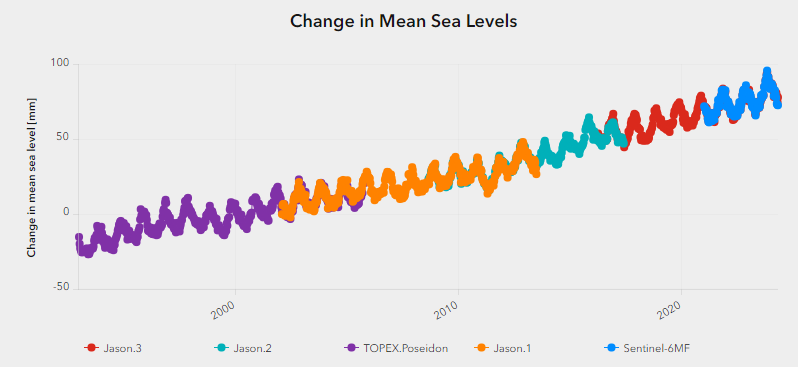
\includegraphics[width=0.8\textwidth]{pictures/sea_levels.png}
    \caption{Change in Mean Sea Levels Over Time.}
    \label{fig:sea_levels}
\end{figure}

The shifts in the general sea level annually across different sea regions are presented in the bar graph in figure \ref{fig:sea_levels2}. The Baltic Sea has the highest average rise, while the South China and North Pacific seas occupy the second and third places, respectively. Such differences demonstrate the variations of the sea level rise effect where the aspects including ocean currents, melting land ice and climate within the region define the effects on the sea level.

\begin{figure}[ht!]
    \centering
    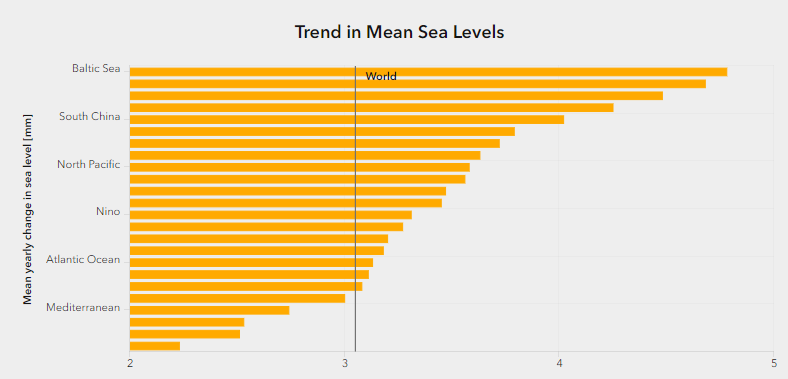
\includegraphics[width=0.9\textwidth]{pictures/sea_levels2.png}
    \caption{Trend in Mean Sea Levels by Region.}
    \label{fig:sea_levels2}
\end{figure}

The final chart in Figure \ref{fig:co2_conc} presents the monthly atmospheric \(\text{CO}_2\) concentrations from 2000 to 2021. The data indicates a steady and significant increase in CO2 levels, with seasonal variations superimposed on this trend. This increase in CO2 concentrations is a primary driver of global warming, reinforcing the urgent need for effective climate policies and mitigation strategies.

In figure \ref{fig:co2_conc}, the monthly average concentration of the atmospheric \(\text{CO}_2\) from the year 2000 to the year 2021 is shown. The \(\text{CO}_2\) level reveals an increasing trend and distinctly higher values for each of the years and months irrespective of the seasonal variation. An important contribution of \(\text{CO}_2\) to the process of global warming shows the need to establish effective climate policies and strategies to limit its effects.

\begin{figure}[ht!]
    \centering
    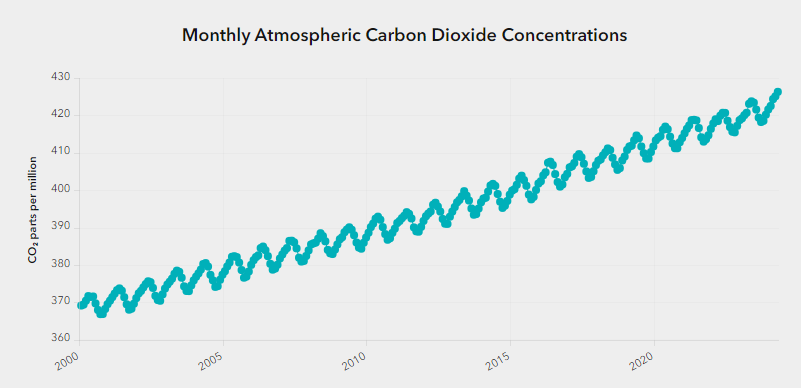
\includegraphics[width=0.8\textwidth]{pictures/co2_conc.png}
    \caption{Monthly Atmospheric Carbon Dioxide Concentrations.}
    \label{fig:co2_conc}
\end{figure}

\subsection{Answer: 1}

Regarding the first question. Strong positive correlation is found between atmospheric \(\text{CO}_2\) levels and sea level. Going by what has been experienced, \(\text{CO}_2\) levels have continued to rise and so has the sea level. This result is due to the greenhouse effect because higher level of \(\text{CO}_2\) increases the heat trapped, thereby the sea expands thermally and glaciers in addition to ice caps melt. The scatter plot in Figure \ref{fig:co2_vs_sea_level} illustrates the correlation between atmospheric \(\text{CO}_2\) concentration and sea level rise.

\begin{figure}[ht!]
    \centering
    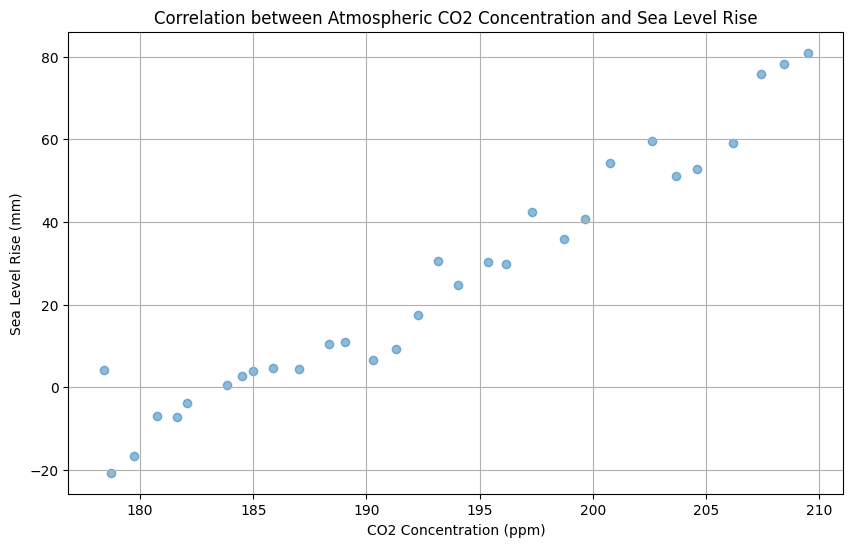
\includegraphics[width=0.7\textwidth]{pictures/q1.png}
    \caption{Correlation between Atmospheric \(\text{CO}_2\) Concentration and Sea Level Rise}
    \label{fig:co2_vs_sea_level}
\end{figure}


\subsection{Answer: 2}
The was no correlation found in between average surface temperatures and the changes in land cover. Despite the assumption that with rising temperatures of the climate, greater changes in the land cover would be observed, it was not the case here. These could be due to reasons such as; climate policies and their application in different regions, the practices of land use, and the capability of certain ecosystems in accommodating the changes in temperature. The scatter plot in Figure \ref{fig:temp_vs_land_cover} shows the correlation between the Z-score normalized mean surface temperature change and land cover change.

\begin{figure}[ht!]
    \centering
    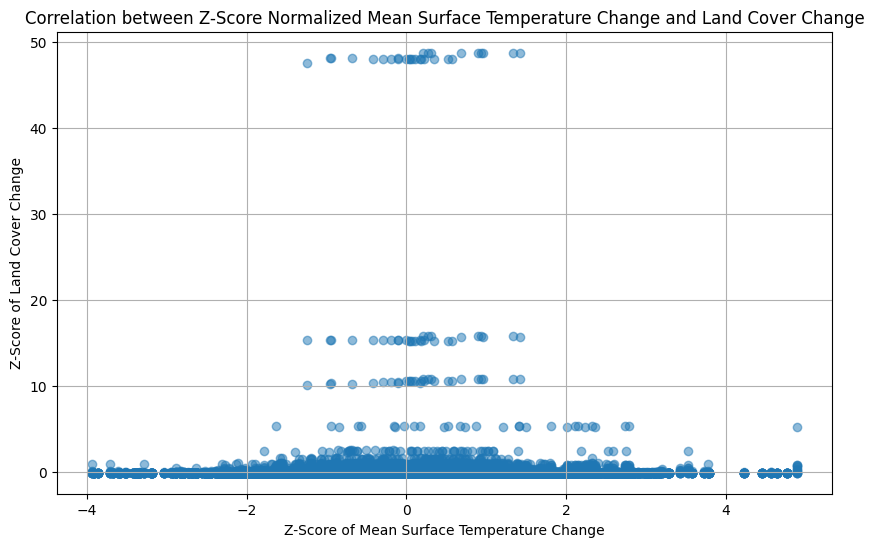
\includegraphics[width=0.7\textwidth]{pictures/q2.png}
    \caption{Correlation between Z-Score Normalized Mean Surface Temperature Change and Land Cover Change}
    \label{fig:temp_vs_land_cover}
\end{figure}

\section*{Conclusions}

The study was able to find an evident correlation between the extent of increase in \(\text{CO}_2\) concentrations in the atmosphere and an equivalent raise in the global sea level implying the impact of greenhouse gases to oceans. However, the anticipated positive correlation between rising temperatures and variations in the land cover was not conclusive, meaning there might other factors that influences those changes. They further, contributes significantly to the formulation of strategies that should be adopted for the mitigation of climate change. Despite the fact that there is considerable evidence of the correlation between \(\text{CO}_2\) levels and sea levels there is an utmost lack of such links with changes in land cover; therefore, one needs to deepen the investigation more to identify the causes. The drawback of this approach is that it may be affected by data quality problems and that the existence of refined data is needed to properly analyze regional differences.

\bibliographystyle{plain}
\bibliography{references}

\end{document}
